\section {Stadiul actual al tehnologiilor utilizate pentru dezvoltarea soluției}

Dezvoltarea unui sistem \acrshort{iot} de automatizare presupune atat o parte hardware cat si una software. Pentru controlarea hardware-ului de la distanta este nevoie de un canal de comunicatii prin care sa se i trimita comenzi. In general, in cazul sistemelor embedded de acest tip folosesc un microcontroller sau un microprocesor care implementeaza stiva \acrshort{ip}.

O alta abordare populara in proiectarea acestor sisteme este dezvoltarea unui controller conectat la internet care are rolul de a colecta informatii de la alte dispozitive din incinta compatibile cu protocolul sau. Mai departe, informatiile colectate sunt transmise unui server spre a fi preprocesate, agregate, oferind utilizatorului date relevante momentului respectiv.

In functie de complexitatea solutiei, partea responsabila pentru procesarea evenimentelor poate varia de la un simplu server conectat la o baza de date pana la un cluster de big-data compus din sute de noduri capabile sa ruleze algoritmi de agregare distribuiti.


\subsection {Apple, Amazon, Google}

Potrivit articolului \cite{AppleRebuildsSiriMesos}, Apple foloseste Apache Mesos, un manager open-source pentru clustere de computatie capabil sa scaleze pana la zeci de mii de noduri pentru a rula serviciile necesare asistentului inteligent Siri intr-o maniera care ofera redundanta la eroare. Urmatorul nivel de integrare vine de la compania Amazon, care ruleaza algoritmii asistenutlui sau inteligent Alexa pe platforma sa de servicii web, \acrfull{aws}. Intr-o maniera similara putem specula ca o companie precum Google foloseste tehnologia sa de orchesterare pentru clustere de computatie, Kubernetes, pentru a rula serviciile necesare Google Assistant.

Toate aceste solutii includ integrari cu sisteme \acrshort{iot} precum lumini inteligente, aspiratoare autonome sau incuietori inteligente au o complexitare ridicata, justificand necesitatea unui cluster computational distribuit. 

\subsection {Espressif}

Espressif Systems ofera o abordare alternativa problemei, prin protocolul de comunicatii Esspressif care compacteaza 5 layere din stiva \acrfull{osi} intr-unul singur, reducand latenta cauzata de pierderea pachetelor in retele congestionate. Fiind mai simplu, iroseste mai putini cicli ai microprocesorului si consuma mai putina memorie. Pentru a permite interactiunea senzorilor si actorilor Esspressif cu dispozitive mobile care nu implementeaza acest protocol este nevoie de un gateway care sa realizeze traducerea pachetelor intre cele doua retele, insa acest lucru este optional.

\begin{figure}[h!]
  \centering
  \fbox {
    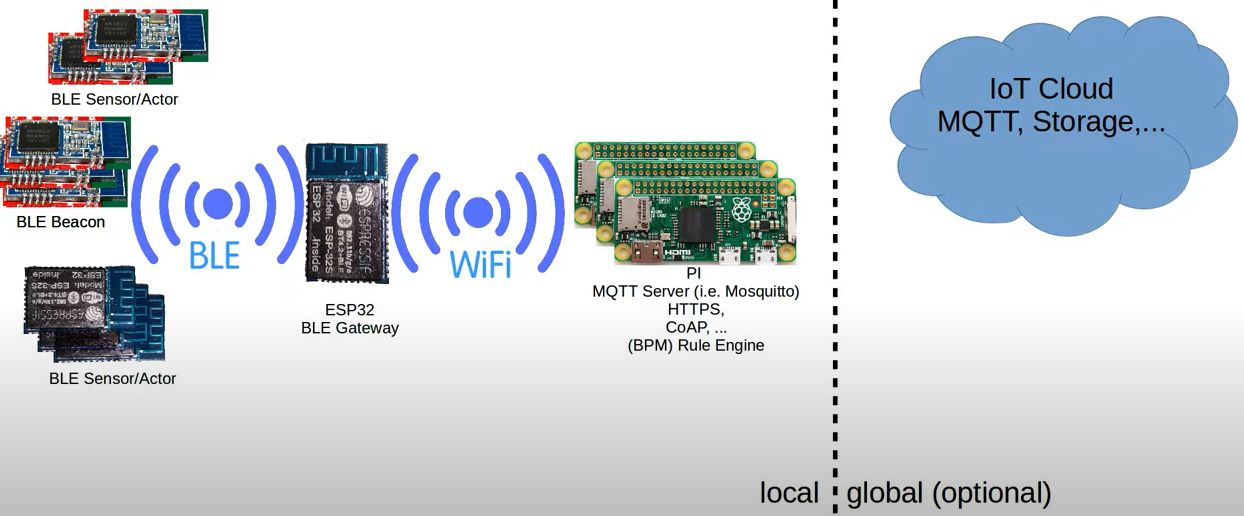
\includegraphics[width=0.6\textwidth]{03/01_espressif_gateway.png}  
  }
  \caption{Sistem interconectare actori Espressif la internet \cite{StackOverflow2021Espressif}}
\end{figure}

Din perspectiva utilizatorului, dispozitivele noi necesita un pas de imperechere in retea, dupa acest pas fiind complet autonome. Chiar daca frameworkul ofera functii ajutatoare pentru criptarea informatiilor transmise, aplicatiile pot alege sa implementeze metoda standard Curve25519, sa isi implementeze propriul mecanism de criptare sau chiar sa o dezactiveze complet.

Proiectandu-ne propriul sistem, beneficiem de libertate in modelarea problemei si alegerea protocoalelor de comunicare. Asadar, se poate concepe un sistem \acrshort{iot} care sa ofere un set de functionalitati mai restrans, folosind hardware disponibil consumatorilor de rand si tehnologii software open-source.

Aditional, pentru o integrare minimala cu unul din asistentii personali mentionati mai sus, de obicei este pus la dispozitia dezvoltatorilor un API bazat pe webhook-uri. Acesta sarcina presupune implementarea unor servicii \acrshort{rest} pe baza unor specificiatii prestabilite. 

\section {Prezentarea tehnologiilor si platformelor de dezvoltare alese}

\subsection {Hardware}

Deoarece proiectul necesita atat interactiunea cu sisteme electrice cat si cu sisteme digitale precum stiva \acrshort{ip}, am ales placa de dezvoltare "Raspberry Pi 3 Model B Rev 1.2". Aceasta ofera un procesor quad core cu arhitectura armv7 de 1.2 Ghz, 1 GB RAM si 26 de pini \acrfull{gpio} pentru interactiunea cu terminalul \acrshort{pots}.

Considerand complexitatea relativ scazuta a circuitului electric, pentru proiectarea \acrshort{pcb} am ales Fritzing, un soft open-source de \acrfull{cad}. Spre deosebire de un program mai profesionist precum Eagle, Fritzing este usor de folosit si dispune de o librarie care contine majoritatea componentelor anologice si digitale. In cazul in care nu exista model pentru o componenta, utilizatorul are posibilitatea de a crea un model din poze si masuratori. 

\subsection {Backend}

Intr-un studiu anual realizat de Stack Overflow, peste 80,000 de dezvoltatori software au ales JavaScript ca cel mai folosit limbaj de programare pentru al noualea an consecutiv. NodeJS a urcat pe locul 5 in popularitate, in timp ce Typescript este pe locul 6. Datorita cerintei de portabilitate am ales NodeJS ca limbaj pentru implementarea serverului aplicatiei. \cite{StackOverflow2021Survey}

Printre alternative viabile pentru acest tip de proiect se numara Java, C\# sau Python, limbaje aflate in primele 10 in topul celor de la Stack Overflow.

Ca framework de dezvoltare a serverului am ales NestJS, oferind o arhitectura \acrfull{mvc} si multe functionalitati convenabile precum:

\begin{itemize}
  \item Framework de injectare a dependintelor: graful (aciclic) de dependinte al aplicatiei este calculat la pornire, fiecarui modul ii sunt satisfacute dependintele, instantiindu-se obiectele necesare o singura data. Daca sunt detectati cicli in graful de dependinte sau nu exista informatii despre cum se poate instantia o clasa, atunci se va arunca o eroare de runtime si aplicatia va iesi cu un status code de eroare. 
  \item Separarea logicii de control a aplicatiei de interfata si de date. Utilizatorul interactioneaza cu interfata, care notifica controllerul de actiunile utilizatorului, controllerul executa logica aplicatiei si actualizeaza modelul corespunzator, schimbari ce se vor reflecta in interfata.
  \item Imbina elemente de \acrfull{oop}, \acrfull{fp} si \acrfull{frp}. De exemplu: modulele si serviciile sunt clase, iar decoratorii claselor sunt functii care modifica comportamentul functiilor adnotate prin compunere.

\end{itemize}

\subsection {Baza de date}

Din punct de vedere al scalabilitatii, pradigma relationala scaleaza vartical (putine servere puternice), pe cand cea nerelationala este orizontala (multe servere mici). Prin urmare am ales MongoDB, o solutie de tip NoSQL rulata in modul "cluster" pentru a oferi redundanta datelor prin replicarea lor de 3 ori pe noduri diferite fizic.

Deoarece MongoDB are nevoie de suport pentru 64 biti, nu poate fi instalata pe acelasi Raspberry Pi unde va rula si serverul. Pentru simplitudine, am ales un serviciu online de hosting gratis, numit Mongo Atlas. Asadar, serverul NodeJS trebuie sa tina cont de eventuala latenta mai ridicata in comunicarea cu baza de date si retransmiterea comenzilor in cazul in care niciunul din nodurile clusterului nu este disponibil.

\subsubsection {Object Document Mapping}

Pentru transformarea si validarea obiectelor de JavaScript in documente ce vor fi stocate in baza de date, am ales Mongoose.

\subsection {Client}

Android este o platforma mobile care s-a maturizat pe parcusul a 12 versiuni majore si principalul competitor de piata al iOS. Avand experienta anterioara ca programator Android si in special cu limbajul de programare Java, a fost o alegere convenabila pentru un prototip rapid.
Este de mentionat ca aceasta alegere de platforma este pur subiectiva, un client similar putand fi dezvoltat pentru iOS sau cu o tehnologie care suporta cross-compilation cum ar fi React Native sau Ionic.
